% Section gramar and basics 
\section{Modellierung einer Mondlandung}
\label{sec:modeling-luna-landing}

\subsection{Simulink Modell der Mondlandung}
\label{sec:sub-simulink-model-luna-landing}
Die Abbildung \ref{fig:simulink-model-luna-landing} zeigt das implementierte Modell der Mondlandung.
\begin{figure}[h]
	\centering
	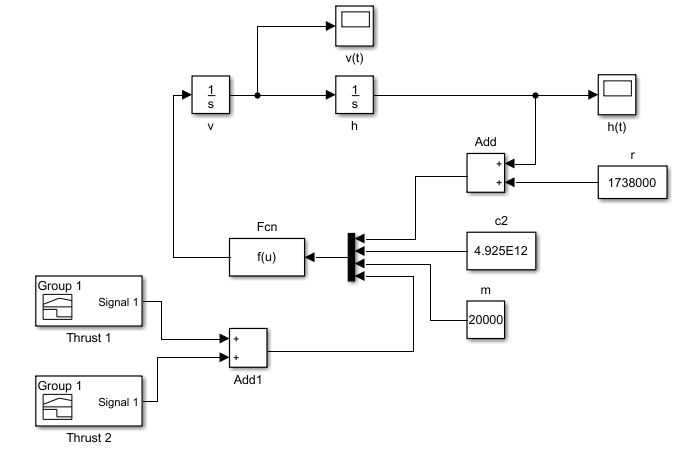
\includegraphics[scale=0.6]{\imageDir/simulink-model-luna-landing.JPG}
	\caption{Simulink Modell der Mondlandung}
	\label{fig:simulink-model-luna-landing}
\end{figure}
-0.008801562	-7.17180995

\subsubsection{Test 1}
\begin{figure}[h]
	\centering
	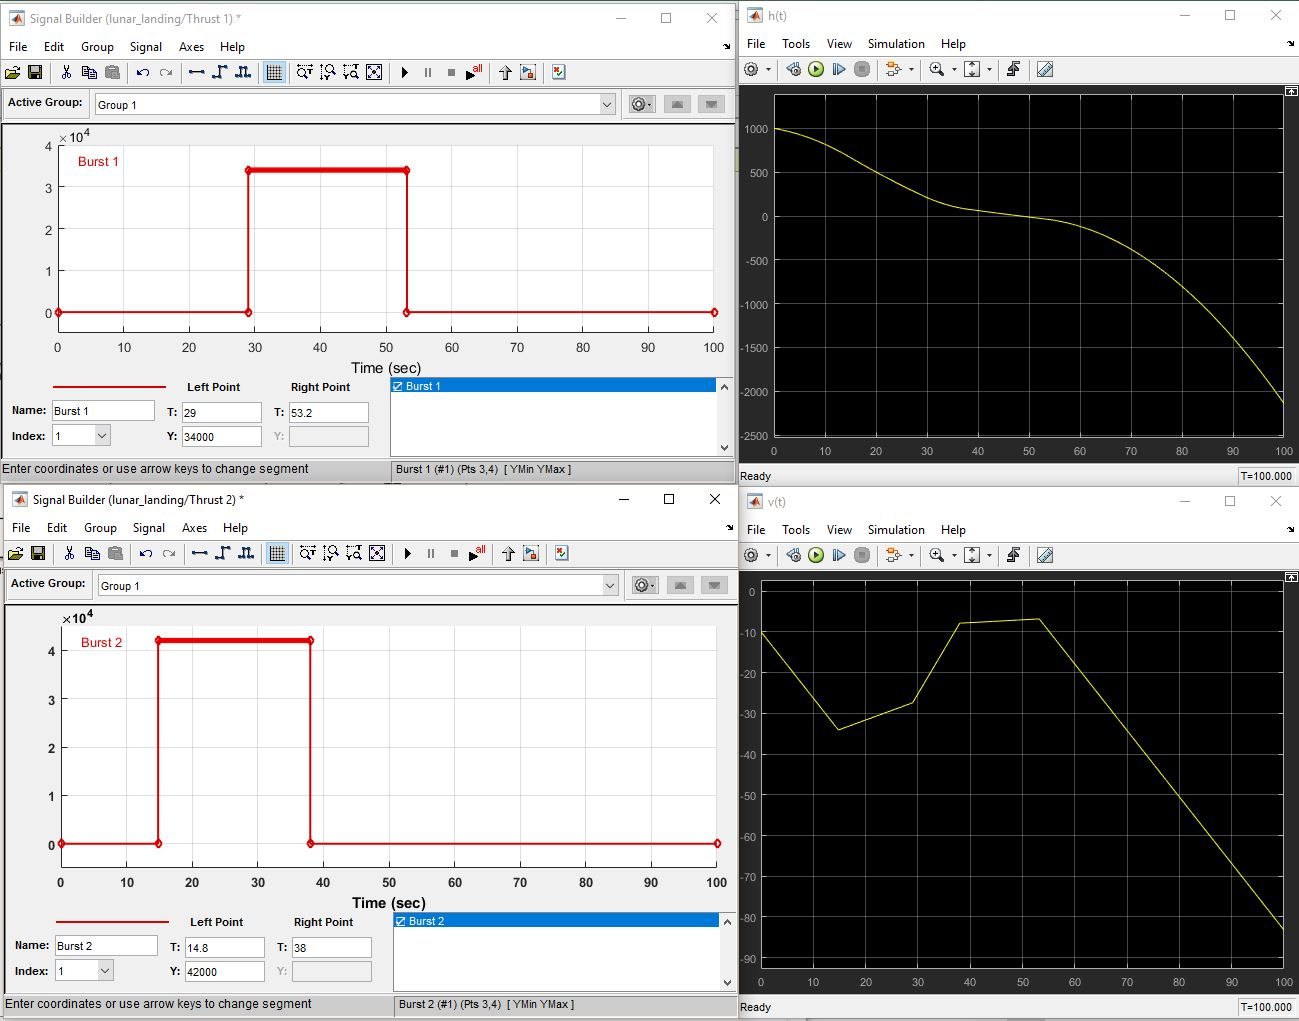
\includegraphics[scale=0.3]{\imageDir/simulink-luna-landing-test-1.JPG}
	\caption{$h_{(t)}$=~-0.0088 $m$, $v_{(t)}$=~-7.17 $m/s$}
	\label{fig:simulink-luna-landing-test-1}
\end{figure}
\ \newpage

\subsubsection{Test 2}
\begin{figure}[h]
	\centering
	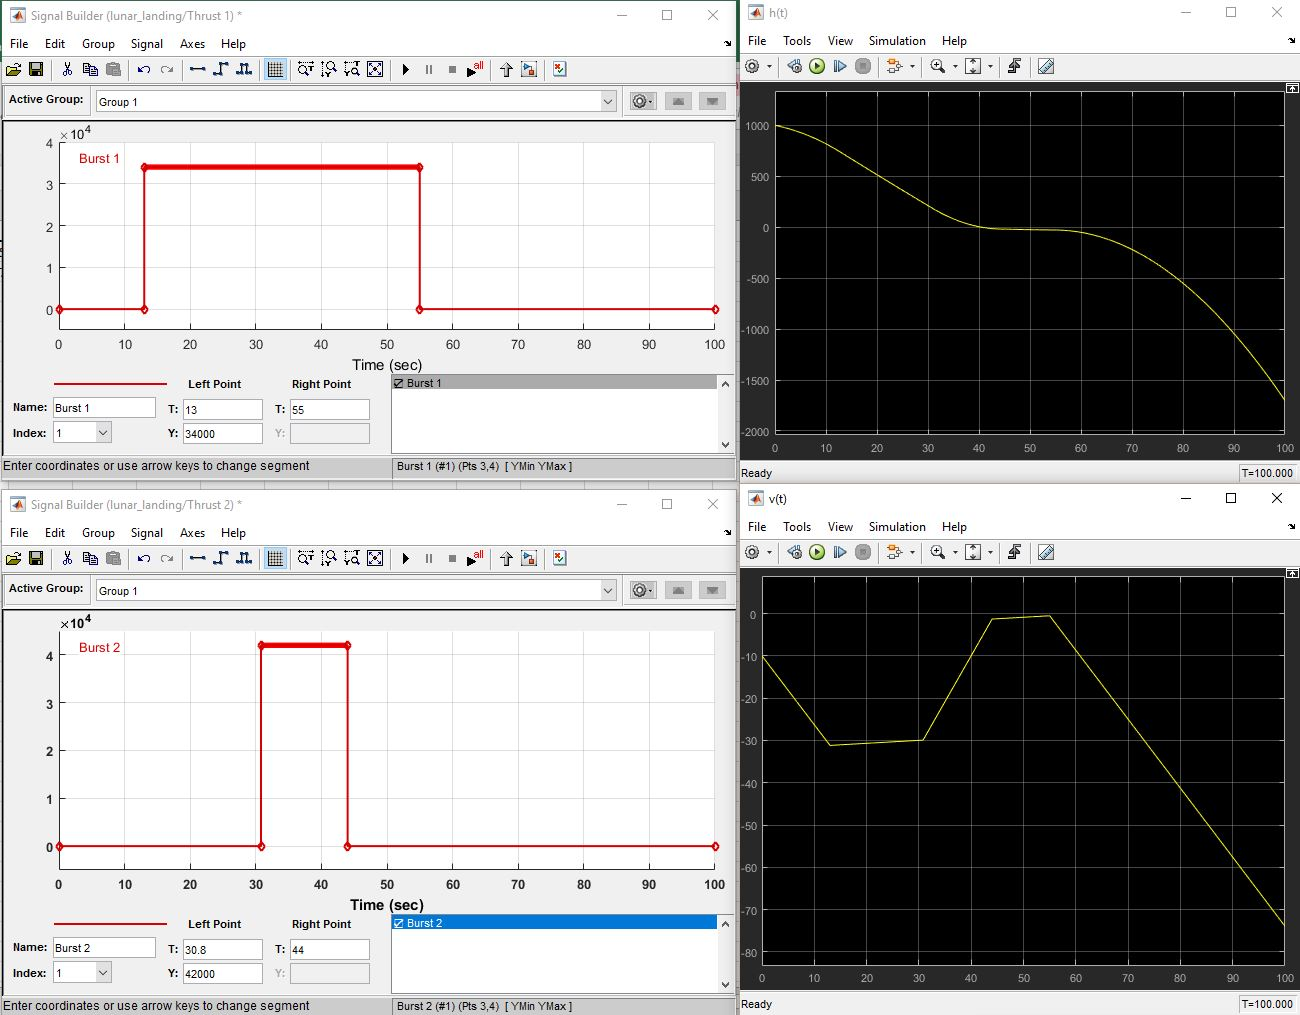
\includegraphics[scale=0.3]{\imageDir/simulink-luna-landing-test-2.JPG}
	\caption{$h_{(t)}$=~-0.0256 $m$, $v_{(t)}$=~-8.72 $m/s$}
	\label{fig:simulink-luna-landing-test-2}
\end{figure}

\subsubsection{Test 3}
\begin{figure}[h]
	\centering
	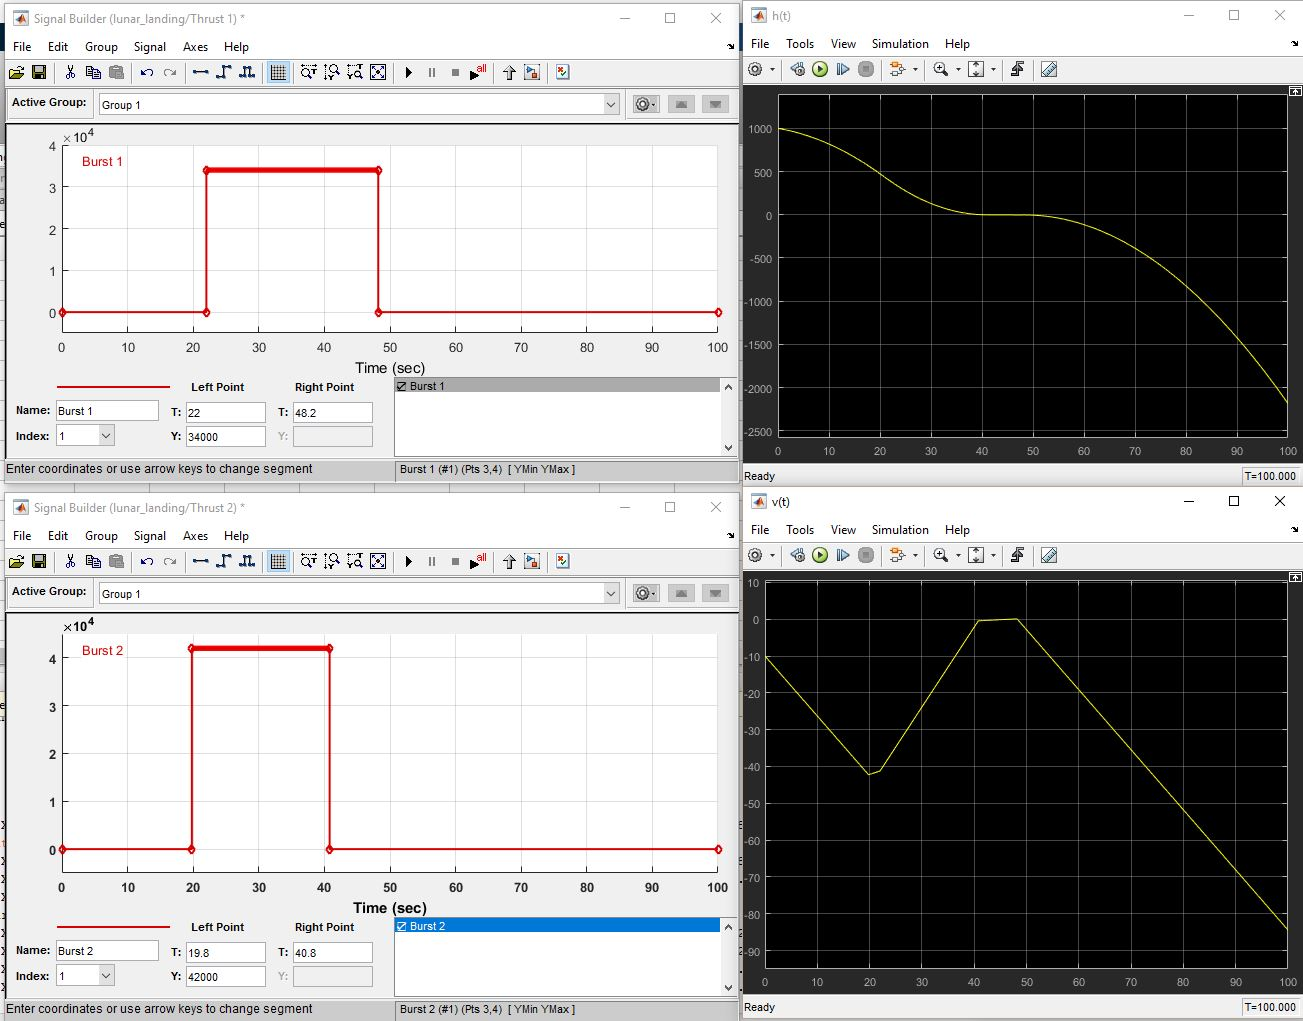
\includegraphics[scale=0.3]{\imageDir/simulink-luna-landing-test-3.JPG}
	\caption{$h_{(t)}$=~-0.0018 $m$, $v_{(t)}$=~-1.44 $m/s$}
	\label{fig:simulink-luna-landing-test-3}
\end{figure}
\ \newpage

\subsubsection{Testergebnisse}
\label{sec:simulink-luna-landing-test-results}
\begin{figure}[h]
	\centering
	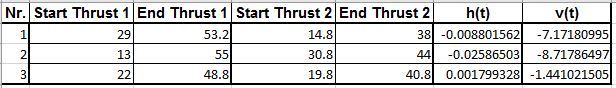
\includegraphics[scale=0.8]{\imageDir/simulink-luna-landing-test-results.JPG}
	\caption{Tabelle mit den Gesamtergebnissen}
	\label{fig:simulink-luna-landing-test-result}
\end{figure}


\subsection{Solver Modifikationen}
\label{sec:sub-simulink-solver-luna-landing}
Als Beispiel wird der Lösungskandidat aus Abschnitt \ref{sec:simulink-luna-landing-test-results} herangezogen, mit dem gezeigt wird, wie sich die Änderungen an den Einstellungen auswirken.

\subsubsection{Test Schrittweite 1 und 0.01}
\begin{figure}[h]
	\centering
	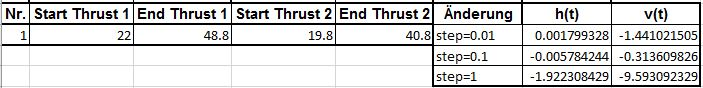
\includegraphics[scale=0.8]{\imageDir/simulink-luna-landing-solver-test-1.JPG}
	\caption{Testergebnisse mit den drei Schrittweiten 0.01, 0.1 und 1}
	\label{fig:simulink-luna-landing-solver-test-1-1}
\end{figure}
\ \newline
Die gravierenden Unterschiede entstehen, da mit einer zu großen Schrittweite schnelle Veränderungen im System nicht erkannt werden können. Bei schnellen Veränderungen im System ist eine kleine Schrittweite von Vorteil, bei langsamen Veränderungen eine große Schrittweite.

\subsubsection{Test verschiedener Integrationsmethoden}
\begin{figure}[h]
	\centering
	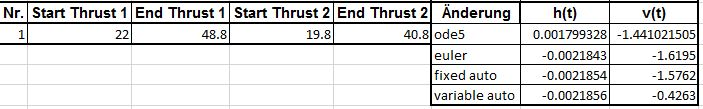
\includegraphics[scale=0.8]{\imageDir/simulink-luna-landing-solver-test-2.JPG}
	\caption{Testergebnisse mit den vier Integrationsmethoden}
	\label{fig:simulink-luna-landing-solver-test-1-1}
\end{figure}
\ \newline
Die verschiedenen Integrationsmethoden \emph{ode5}, \emph{euler} unterscheiden sich durch ihren lokalen und globalen Error. Diese Error Indikatoren werden  durch verschiedene Mechanismen die bei der Integration angewandt werden, wie gewichtetes Mittel, Miteinbeziehung von vorherigen und/oder geschätzten Nachfolgern und der Verwendung empirischer Faktoren, beeinflusst.
\newpage

\subsection{Modifikation der Mondlandungsmodell}
\label{sec:sub-simulink-modified-model-luna-landing}

Die Abbildung zeigt das modifizierte Modell der Mondlandung.
\begin{figure}[h]
	\centering
	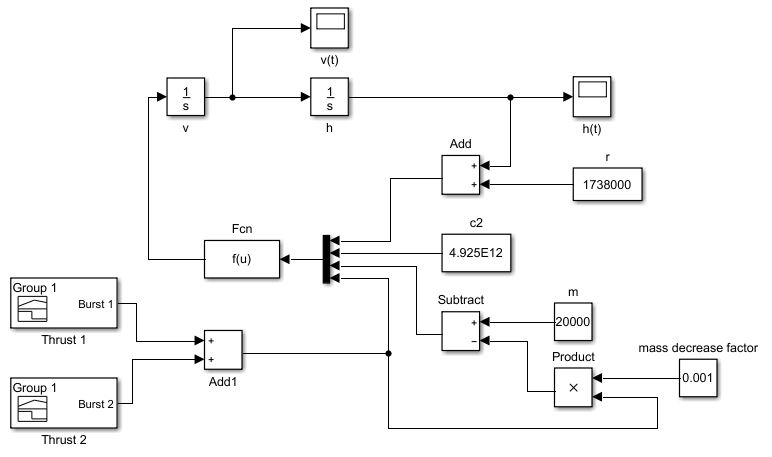
\includegraphics[scale=0.8]{\imageDir/simulink-model-luna-landing-modified.JPG}
	\caption{Mondladungsmodell mit Massenreduktion beim Bremsen}
	\label{fig:simulink-luna-landing-modified}
\end{figure}

\subsubsection{Test 1}
\subsubsection{Test 2}
\subsubsection{Test 3}
\subsubsection{Test 4}
\subsubsection{Test 5}

\newpage
\section{Optimierung mit einen Evolutionsalgorithmus}
\subsection{Der Evolutionsalgorithmus}

\begin{code}
	\caption{Funktion die einen Lösungskandidaten initialisiert}
	\mSourceFile{\srcDir/initialize.m}
	\label{fig:initialize-m}
\end{code}

\begin{code}
\caption{Funktion, welche die Mutanten aus einem Elter erzeugt}
\mSourceFile{\srcDir/bread.m}
\label{fig:bread-m}
\end{code}

\begin{code}
\caption{Funktion, welche einen Elter zu einem Mutanten konvertiert}
\mSourceFile{\srcDir/mutate.m}
\label{fig:mutate-m}
\end{code}

\begin{code}
\caption{Funktion, welche die Simulation für einen Lösungskandidaten durchführt}
\mSourceFile{\srcDir/evaluate.m}
\label{fig:evaluate-m}
\end{code}

\begin{code}
\caption{Funktion, welche die Simulation für einen Lösungskandidaten durchführt}
\mSourceFile{\srcDir/moonLanding.m}
\label{fig:moon-landing-m}
\end{code}

\newpage
\subsection{Optimierungen des Evolutionsalgorithmus}
\subsubsection{Was ist eine geeignete Fitnessfunktion ?}
\subsubsection{Was muss optimiert werden ?}
\subsubsection{Welche Parameter können modifiziert werden ?}
\subsubsection{Warum ein Evolutionsalgorithmus ?}

\newpage
\subsection{Auswertung der Testfälle}
\subsubsection{Test 1}
\subsubsection{Test 2}
\subsubsection{Test 3}
\subsubsection{Test 4}
\subsubsection{Test 5}
\subsubsection{Gegenüberstellung der Tests}